%% Преамбула TeX-файла

% 1. Стиль и язык
\documentclass[utf8x, 14pt]{G7-32} % Стиль (по умолчанию будет 14pt)

% Остальные стандартные настройки убраны в preamble.inc.tex.
\include{preamble.inc}

% Настройки листингов.
\include{listings.inc}

% Полезные макросы листингов.
\include{macros.inc}

% Стиль титульного листа и заголовки

%\NirEkz{Экз. 3}                                  % Раскоментировать если не требуется
%\NirGrif{Секретно}                % Наименование грифа

%\gosttitle{Gost7-32}       % Шаблон титульной страницы, по умолчанию будет ГОСТ 7.32-2001, 
% Варианты GostRV15-110 или Gost7-32 
 
\NirOrgLongName{Правительство Российской Федерации\par
САНКТ-ПЕТЕРБУРГСКИЙ ГОСУДАРСТВЕННЫЙ УНИВЕРСИТЕТ\par
%Факультет прикладной математики --- процессов управления
Направление 01.03.02 «Прикладная математика и информатика»\par
Кафедра технологии программирования 
}                                           %% Полное название организации

\NirUdk{\hspace{1em}}
\NirGosNo{\hspace{1em}}
\NirInventarNo{\hspace{1em}}

%\NirConfirm{Согласовано}                  % Смена УТВЕРЖДАЮ
\NirBoss[.49]{}{}            %% Заказчик, утверждающий НИР


%\NirReportName{Научно-технический отчет}   % Можно поменять тип отчета
%\NirAbout{О составной части \par опытно-конструкторской работы} %Можно изменить о чем отчет

%\NirPartNum{Часть}{1}                      % Часть номер

%\NirBareSubject{}                  % Убирает по теме если раскоментить

% \NirIsAnnotacion{АННОТАЦИОННЫЙ }         %% Раскомментируйте, если это аннотационный отчёт
%\NirStage{промежуточный}{Этап \No 1}{} %%% Этап НИР: {номер этапа}{вид отчёта - промежуточный или заключительный}{название этапа}
%\NirStage{}{}{} %%% Этап НИР: {номер этапа}{вид отчёта - промежуточный или 

%\Nir{АВТОМАТИЗИРОВАННОЕ ТЕСТИРОВАНИЕ С ПОМОЩЬЮ DEEP LEARNING В GAME DEV}

\NirSubject{АВТОМАТИЗИРОВАННОЕ ТЕСТИРОВАНИЕ С ПОМОЩЬЮ DEEP LEARNING В GAMEDEV}                                   % Наименование темы
\NirFinal{}                        % Заключительный, если закоментировать то промежуточный
\finalname{~\hspace{-100em}~}               % Название финального отчета (Заключительный) 
%\NirCode{Шифр\,---\,САПР-РЛС-ФИЗТЕХ-1} % Можно задать шифр как в ГОСТ 15.110
\NirCode{}

\NirManager{Научный руководитель}{\hspace{2.1em}канд. техн. наук, доцент\\ \hspace{26.5em}И.С.~Блеканов} %% Название руководителя
\NirIsp{Работу выполнил}{\hspace{7.2em}гр. 20.Б08-пу,\\\hspace{28.3em}М.~Павлов} %% Название руководителя

\NirYear{2022}%% если нужно поменять год отчёта; если закомментировано, ставится текущий год
\NirTown{Санкт-Петербург}                           %% город, в котором написан отчёт


\usepackage{spacingtricks}


\begin{document}

\frontmatter % выключает нумерацию ВСЕГО; здесь начинаются ненумерованные главы: реферат, введение, глоссарий, сокращения и прочее.

\maketitle %создает титульную страницу


%\begin{executors}
%\personalSignature{Первый исполнитель}{ФИО}

%\personalSignature{Второй исполнитель}{ФИО}
%\end{executors}


%\listoffigures                         % Список рисунков

%\listoftables                          % Список таблиц

%\NormRefs % Нормативные ссылки 
% Команды \breakingbeforechapters и \nonbreakingbeforechapters
% управляют разрывом страницы перед главами.
% По-умолчанию страница разрывается.

% \nobreakingbeforechapters
% \breakingbeforechapters

%\include{00-abstract}

\begin{spacing}{1.5}

\tableofcontents

\printnomenclature % Автоматический список сокращений

\Introduction

Целью работы является создание всякой всячины. Для достижения поставленной цели необходимо решить следующие задачи:

\begin{itemize}
\item проанализировать существующую всячину;
\item запрограммировать свою, новую всячину;
\item проверить её работоспособность.
\end{itemize}
%
%Проверяем как у нас работают сокращения, обозначения и определения "---
%MAX, 
%\Abbrev{MAX}{Maximum ""--- максимальное значение параметра}
%API 
%\Abbrev{API}{application programming interface ""--- внешний интерфейс взаимодействия с приложением}
%с обратным прокси.
%\Define{Обратный прокси}{тип прокси-сервера, который ретранслирует}





\mainmatter % это включает нумерацию глав и секций в документе ниже

\chapter{Постановка задачи}
\label{cha:analysis}
%
% % В начале раздела  можно напомнить его цель
%

Перед началом научно-исследовательской работы был проанализирован ряд статей, посвященных применению методов глубокого обучения для таких жанров игр, как FPS (шутеры от первого лица) \cite{bergdahl2020augmenting}, прятки \cite{baker2019emergent}, а также аркадные и гоночные игры \cite{tufano2022using}.

\section{Среда}

В качестве среды для работы была выбрана платформа \textit{Gym} на языке Python \cite{Gym} по следующим причинам:
\begin{itemize}
	\item[--] в \textit{Gym} представлен ряд встроенных игр, которые можно использовать для тестирования моделей;
	\item[--] \textit{Gym} выступает в качестве посредника между игровой средой и агентом (моделью), выполняя нужные команды и собирая информацию о состоянии среды на каждом шаге.
\end{itemize}

Среди игровых сред, входящих в \textit{Gym}, была выбрана Lunar Lander v2 \cite{lunarlanderv2}. В ней игроку или агенту предлагается посадить лунный лендер (посадочный модуль) на заданную площадку, обозначенную флагами. Игра начинается с того, что центру масс модуля, находящегося наверху экрана, сообщается случайная сила. На каждом моменте времени можно привести в действие один трех двигателей: левый, правый или основной, либо ничего не делать. Игровой эпизод заканчивается, если лендер совершает посадку или покидает область видимости.

\section{Архитектура}

В научной литературе, прочитанной в рамках исследовательской работы, наиболее часто используемым алгоритмом являлся Deep Q-Network (DQN). Задача данного алгоритма "--- формирование функции полезности \(Q\), заданную следующим уравнением Беллмана: \[Q(s_t, a_t) \leftarrow Q(s_t, a_t) + \alpha \cdot (r(s_t, a_t) + \gamma \cdot \max_a Q(s_{t+1}, a) - Q(s_t, a_t)),\] где 
\begin{itemize}
	\item[--] \(s_t\) "--- состояние среды в момент времени \(t\); 
	\item[--]  \(a_t\) "--- действие агента, совершенное в момент времени \(t\);
	\item[--] \(r(s_t, a_t)\) "--- награда, полученная при переходе из состояния \(s_t\) в состояние \(s_{t+1}\);
	\item[--] \(\alpha \in (0, 1]\) "--- скорость обучения;
	\item[--] \(\gamma \in [0, 1]\) "--- дисконтирующий множитель; чем ближе он к единице, тем больше моделью будет учитываться награда в последующих состояниях.
\end{itemize}

Исследование агентом новых состояний и действий происходит благодаря $\varepsilon$-жадной стратегии принятия решений. Все они записываются в буфер воспроизведения (replay buffer), откуда на каждом шаге случайным образом выбирается партия из \(n\) кортежей вида \((s_t, a_t, r(s_t, a_t), s_{t+1})\).

В DQN используются две нейросети: одна отвечает за оценку \(Q\) для текущего состояния и обновляется на каждом шаге, когда как другая вычисляет оптимальное значения \(Q\) для последующего состояния (её веса изменяются периодически).

В качестве функции потерь была выбрана функция Хьюбера, т.~к. она является менее чувствительной к выбросам, нежели среднеквадратическая ошибка (MSE).

Для достижения большей стабильности при обучении использовалась модификация стандартного алгоритма DQN, называемая Dueling Double Deep Q-Network (D3QN) \cite{wang2016dueling,hasselt2016deep}. Кривая обучения такой модели представлена на рис.~\ref{fig:trainScore}

\begin{figure}
	\centering
	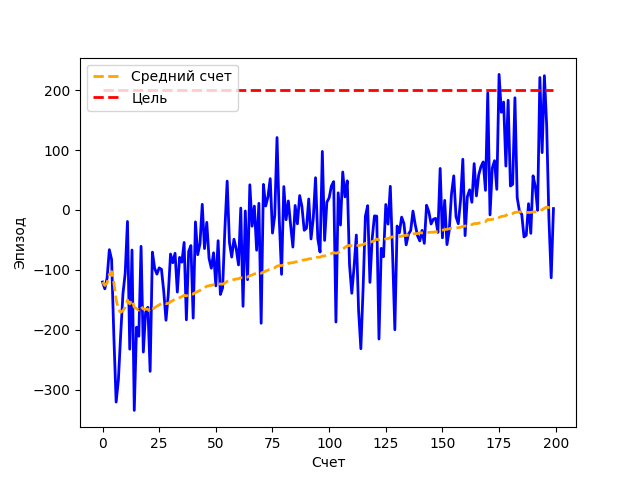
\includegraphics[width=\textwidth]{figures/d3qn_train_score}
	\caption{Пример кривой обучения D3QN в среде Lunar Lander v2.}
	\label{fig:trainScore}
\end{figure}

%Кстати, про картинки. Во-первых, для фигур следует использовать \texttt{[ht]}. Если и после этого картинки вставляются <<не по ГОСТ>>, т.е. слишком далеко от места ссылки, "--- значит у вас в РПЗ \textbf{слишком мало текста}! Хотя и ужасный параметр \texttt{!ht} у окружения \texttt{figure} тоже никто не отменял, только при его использовании документ получается страшный, как в ворде, поэтому просьба так не делать по возможности.

%\begin{enumerate}
%\item Перечисление с номерами.
%\item Номера первого уровня. Да, ГОСТ требует именно так "--- сначала буквы, на втором уровне "--- цифры.
%Чуть ниже будет вариант <<нормальной>> нумерации и советы по её изменению.
%Да, мне так нравится: на первом уровне выравнивание элементов как у обычных абзацев. Проверим теперь вложенные списки.
%\begin{enumerate}
%\item Номера второго уровня.
%\item Номера второго уровня. Проверяем на длииииной-предлиииииииииинной строке, что получается.... Сойдёт.
%\end{enumerate}
%\item По мнению Лукьяненко, человеческий мозг старается подвести любую проблему к выбору
%  из трех вариантов.
%\item Четвёртый (и последний) элемент списка.
%\end{enumerate}
%
%Теперь мы покажем, как изменить нумерацию на «нормальную», если вам этого захочется. Пара команд в начале документа поможет нам.
%
%\renewcommand{\labelenumi}{\arabic{enumi})}
%\renewcommand{\labelenumii}{\asbuk{enumii})}
%
%\begin{enumerate}
%\item Изменим нумерацию на более привычную...
%\item ... нарушим этим гост.
%\begin{enumerate}
%\item Но, пожалуй, так лучше.
%\end{enumerate}
%\end{enumerate}
%
%В заключение покажем произвольные маркеры в списках. Для них нужен пакет \textbf{enumerate}.
%\begin{enumerate}[1.]
%\item Маркер с арабской цифрой и с точкой.
%\item Маркер с арабской цифрой и с точкой.
%\begin{enumerate}[I.]
%\item Римская цифра с точкой.
%\item Римская цифра с точкой.
%\end{enumerate}
%\end{enumerate}
%
%В отчётах могут быть и таблицы "--- см. табл.~\ref{tab:tabular} и~\ref{tab:longtable}.
%Небольшая таблица делается при помощи \Code{tabular} внутри \Code{table} (последний
%полностью аналогичен \Code{figure}, но добавляет другую подпись).
%
%\begin{table}[ht]
%  \caption{Пример короткой таблицы с коротким названием}
%  \begin{tabular}{|r|c|c|c|l|}
%  \hline
%  Тело      & $F$ & $V$  & $E$ & $F+V-E-2$ \\
%  \hline
%  Тетраэдр  & 4   & 4    & 6   & 0         \\
%  Куб       & 6   & 8    & 12  & 0         \\
%  Октаэдр   & 8   & 6    & 12  & 0         \\
%  Додекаэдр & 20  & 12   & 30  & 0         \\
%  Икосаэдр  & 12  & 20   & 30  & 0         \\
%  \hline
%  Эйлер     & 666 & 9000 & 42  & $+\infty$ \\
%  \hline
%  \end{tabular}
%  \label{tab:tabular}
%\end{table}
%
%Для больших таблиц следует использовать пакет \Code{longtable}, позволяющий создавать
%таблицы на несколько страниц по ГОСТ.
%
%Для того, чтобы длинный текст разбивался на много строк в пределах одной ячейки, надо в
%качестве ее формата задавать \texttt{p} и указывать явно ширину: в мм/дюймах
%(\texttt{110mm}), относительно ширины страницы (\texttt{0.22\textbackslash textwidth})
%и~т.п.
%
%Можно также использовать уменьшенный шрифт "--- но, пожалуйста, тогда уж во \textbf{всей}
%таблице сразу.
%
%\begin{center}
%  \begin{longtable}{|p{0.40\textwidth}|c|p{0.30\textwidth}|}
%    \caption{Пример длинной таблицы с длинным названием на много длинных-длинных строк}
%    \label{tab:longtable}
%    \\ \hline
%    Вид шума & Громкость, дБ & Комментарий \\
%    \hline \endfirsthead
%    \subcaption{Продолжение таблицы~\ref{tab:longtable}}
%    \\ \hline \endhead
%    \hline \subcaption{Продолжение на след. стр.}
%    \endfoot
%    \hline \endlastfoot
%    Порог слышимости             & 0     &                                                \\
%    \hline
%    Шепот в тихой библиотеке     & 30    &                                                \\
%    Обычный разговор             & 60-70 &                                                \\
%    Звонок телефона              & 80    & \small{Конечно, это было до эпохи мобильников} \\
%    Уличный шум                  & 85    & \small{(внутри машины)}                        \\
%    Гудок поезда                 & 90    &                                                \\
%    Шум электрички               & 95    &                                                \\
%    \hline
%    Порог здоровой нормы         & 90-95 & \small{Длительное пребывание на более
%    громком шуме может привести к ухудшению слуха}                                        \\
%    \hline
%    Мотоцикл                     & 100   &                                                \\
%    Power Mower                  & 107   & \small{(модель бензокосилки)}                  \\
%    Бензопила                    & 110   & \small{(Doom в целом вреден для здоровья)}     \\
%    Рок-концерт                  & 115   &                                                \\
%    \hline
%    Порог боли                   & 125   & \small{feel the pain}                          \\
%    \hline
%    Клепальный молоток           & 125   & \small{(автор сам не знает, что это)}          \\
%    \hline
%    Порог опасности              & 140   & \small{Даже кратковременное пребывание на
%    шуме большего уровня может привести к необратимым последствиям}                       \\
%    \hline
%    Реактивный двигатель         & 140   &                                                \\
%                                 & 180   & \small{Необратимое полное повреждение
%                                 слуховых органов}                                        \\
%    Самый громкий возможный звук & 194   & \small{Интересно, почему?..}                   \\
%  \end{longtable}
%\end{center}

%%% Local Variables:
%%% mode: latex
%%% TeX-master: "rpz"
%%% End:

\chapter{Эксперимент}
\label{cha:research}

\section{Ход работы}

В среду были добавлены искусственные баги, которые проявляются при первом посещении агентом областей \(x \in (-0,9; -0.8)\) и \(x \in (0,75; 0.8)\). Эти участки обозначены красным цветом на рис.~\ref{fig:bugLocations}. Интервалы были выбраны так, чтобы они находились вне стандартной траектории посадки и требовали отклонения от курса.

\begin{figure}
	\centering
	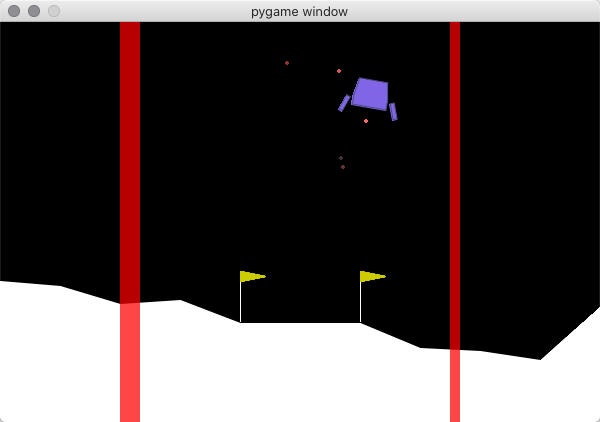
\includegraphics[width=0.75\textwidth]{figures/bug locations}
	\caption{Области проявления багов.}
	\label{fig:bugLocations}
\end{figure}

За первое посещение каждой из областей лендер получает награду в \(+250\) единиц. После этого в этом эпизоде баг не проявляется, и для максимизации награды агенту остается совершить посадку. Первичные тесты показали, что награда при попадании в заданные интервалы плохо мотивировала модель на отклонение от оптимального курса посадки (даже при её увеличении), поэтому было решено добавить штраф в \(-50\) единиц, если агент завершает эпизод, не найдя ни одного бага. Более высокие штрафы здесь не подошли, т.~к. они мотивируют агента вовсе избегать посадки на площадку.

Гиперпараметры модели были подобраны эмпирически с целью достижения исходной моделью среднего счета за последние 100 эпизодов в >200 единиц. Тогда создатели считают среду <<разрешенной>> \cite{lunarlanderv2}.

\section{Результаты эксперимента}

\begin{table}[ht]
	\centering
	\caption{Число эпизодов (из 100), в которых модели нашли хотя бы один баг.}
	\begin{tabular}{ l r r r }
		\hline
		№ & \makecell[r]{Итоговая\\D3QN} & \makecell[r]{Исходная\\D3QN} & Случайный агент \\
		\hline
		1 & 49 & 0 & 22\\
		2 & 38 & 0 & 23\\
		3 & 37 & 0 & 21\\
		4 & 42 & 0 & 20\\
		5 & 42 & 0 & 24\\
		6 & 46 & 0 & 27\\
		7 & 49 & 0 & 26\\
		8 & 39 & 0 & 14\\
		9 & 54 & 0 & 14\\
		10 & 39 & 0 & 19\\
		\hline
		\textit{среднее} & 43,5 & 0 & 21 \\
		\textit{медиана} & 42 & 0 & 21,5 \\
		\textit{ср.~кв.~отклонение} & 5,72 & 0 & 4,447 \\
		\hline
	\end{tabular}
	\label{tab:results}
\end{table}

Полученная модель D3QN тренировалась в течение 250 эпизодов. После этого, натренированный агент дополнительно проходил ещё 100 последовательных эпизодов, записывая число найденных багов на каждом. 

Из-за того, что поверхность Луны и сила, приложенная к центру масс модуля различаются от эпизода к эпизоду, тесты были проведены 10 раз для получения усредненных значений.

Производительность модели сравнивается с исходной D3QN, которая не получала награду за нахождение багов на этапе тренировки, а также с агентом, который на каждом шаге выбирает случайное действие. Результаты эксперимента приведены в табл.~\ref{tab:results}. 

Результаты показывают, что исходная модель D3QN вовсе не справляется с задачей поиска ошибок. Агент модифицированной D3QN смог показать лучший результат среди всех трех: это говорит о том, что награда, полученная за нахождение багов побуждает модель их искать, даже если это негативно влияет на посадку модуля.

%%% Local Variables:
%%% mode: latex
%%% TeX-master: "rpz"
%%% End:

\chapter{Результаты}
\label{cha:results}

\section{Что такого страшного получил?}

В данном разделе приводятся результаты экспериментов.


%%% Local Variables:
%%% mode: latex
%%% TeX-master: "rpz"
%%% End:



\backmatter %% Здесь заканчивается нумерованная часть документа и начинаются ссылки и
            
\Conclusion % заключение к отчёту

В ходе проделанной работы был продемонстрирован подход для автоматизированного тестирования игр с помощью методов глубокого обучения. На примере среды из платформы \textit{Gym} было показано, что метод, награждающий агента в зависимости от нахождения ошибок, показывает лучшие результаты, нежели стандартная Deep Learning-модель.

Итоговый код реализации доступен в открытом репозитории на GitHub \cite{rl4testing}.

Несмотря на полученные результаты, вопрос автоматизированного тестирования требует дополнительных исследований. В дальнейшем следует перейти от искусственных багов к изучению ошибок, возникающих при разработке настоящих продуктов в области GameDev. Это могут быть, например, поиск областей с низкой частотой кадров в секунду (FPS) или участков, где игровой агент может застрять либо, наоборот, свободно пройти там, где это нежелательно. 

%%% Local Variables: 
%%% mode: latex
%%% TeX-master: "rpz"
%%% End: 
%% заключение


\include{81-biblio}


\appendix   % Тут идут приложения

%\include{90-appendix1}

%\include{91-appendix2}

\end{spacing}

\end{document}

%%% Local Variables:
%%% mode: latex
%%% TeX-master: t
%%% End:
